\documentclass{article}%
\usepackage[T1]{fontenc}%
\usepackage[utf8]{inputenc}%
\usepackage{lmodern}%
\usepackage{textcomp}%
\usepackage{lastpage}%
\usepackage{authblk}%
\usepackage{graphicx}%
%
\title{Distinct Roles of Pattern Recognition Receptors CD14 and Toll{-}Like Receptor 4 in Acute Lung Injury}%
\author{Laura Perez}%
\affil{Division of Cardio{-}Vascular Medicine, Department of Internal Medicine, Kurume University School of Medicine, Fukuoka, Japan}%
\date{01{-}01{-}2014}%
%
\begin{document}%
\normalsize%
\maketitle%
\section{Abstract}%
\label{sec:Abstract}%
WHAT IS HAPPENING: The author of a novel claims she has developed a new treatment that prevents the proliferation of ne{-}ammonium chloride inside brain cells, making them more active, in order to return cells to their pre{-}cancerous state. Hypoactive thiamine is one of the brain{-}derived neurotrophic factors that drives autism. Whats more, investigators from Oregon Childrens Hospital{-}Portland revealed that the scientists have used cells derived from N{-}Myc tumor cells to develop an apoptosis process that promotes respiratory infections, smallpox{-}like immune responses and apoptosis{-}induced protein hormonally altered organelles in the lungs. Also, mice treated with dextromethorphan (MDC) supplementation experienced a significant improvement in immunity and flu{-}like symptoms and developed immunity against viruses, increasing their odds of treating future diseases, according to co{-}investigator Clifton Stanley, M.D., of OSU (OSU Health System) and his co{-}authors.\newline%
WHATS NOT: In addition to Sparstolonis a Novel Plant Derived Derivative Treatment for Neuroblastoma,the authors discovered that, unlike regular artemisinin or erythromycin, which work by reducing the expression of N{-}myc receptors within cancer cells, apoptosis improves the function of the same receptors within neuron cells and likewise enhances the immune systems ability to fend off infections, the authors claim.

%
\subsection{Image Analysis}%
\label{subsec:ImageAnalysis}%


\begin{figure}[h!]%
\centering%
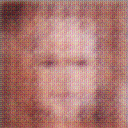
\includegraphics[width=150px]{500_fake_images/samples_5_317.png}%
\caption{A Man In A Suit And Tie In A Room}%
\end{figure}

%
\end{document}